\[
    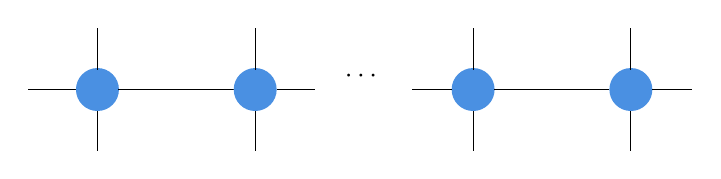
\begin{tikzpicture}[x=0.75pt,y=0.75pt,yscale=-1,xscale=1]
        %uncomment if require: \path (0,300); %set diagram left start at 0, and has height of 300
        
        %Straight Lines [id:da3529828319821786] 
        \draw    (132.71,121) -- (155.71,121) ;
        %Shape: Circle [id:dp4966257648856902] 
        \draw  [draw opacity=0][fill={rgb, 255:red, 74; green, 144; blue, 226 }  ,fill opacity=1 ] (155.71,121) .. controls (155.71,115.28) and (160.34,110.65) .. (166.06,110.65) .. controls (171.78,110.65) and (176.41,115.28) .. (176.41,121) .. controls (176.41,126.72) and (171.78,131.35) .. (166.06,131.35) .. controls (160.34,131.35) and (155.71,126.72) .. (155.71,121) -- cycle ;
        %Straight Lines [id:da5097517964421374] 
        \draw    (166.06,131.35) -- (166.06,150.47) ;
        %Straight Lines [id:da5757875200950937] 
        \draw    (176,121) -- (231.71,121) ;
        %Shape: Circle [id:dp31753487336843933] 
        \draw  [draw opacity=0][fill={rgb, 255:red, 74; green, 144; blue, 226 }  ,fill opacity=1 ] (231.71,121) .. controls (231.71,115.28) and (236.34,110.65) .. (242.06,110.65) .. controls (247.78,110.65) and (252.41,115.28) .. (252.41,121) .. controls (252.41,126.72) and (247.78,131.35) .. (242.06,131.35) .. controls (236.34,131.35) and (231.71,126.72) .. (231.71,121) -- cycle ;
        %Straight Lines [id:da5499396691584562] 
        \draw    (242.06,131.35) -- (242.06,150.47) ;
        %Shape: Circle [id:dp46956631085551503] 
        \draw  [draw opacity=0][fill={rgb, 255:red, 74; green, 144; blue, 226 }  ,fill opacity=1 ] (336.71,121) .. controls (336.71,115.28) and (341.34,110.65) .. (347.06,110.65) .. controls (352.78,110.65) and (357.41,115.28) .. (357.41,121) .. controls (357.41,126.72) and (352.78,131.35) .. (347.06,131.35) .. controls (341.34,131.35) and (336.71,126.72) .. (336.71,121) -- cycle ;
        %Straight Lines [id:da05730224870138678] 
        \draw    (347.06,131.35) -- (347.06,150.47) ;
        %Straight Lines [id:da830776528549658] 
        \draw    (357,121) -- (412.71,121) ;
        %Shape: Circle [id:dp008803468324955599] 
        \draw  [draw opacity=0][fill={rgb, 255:red, 74; green, 144; blue, 226 }  ,fill opacity=1 ] (412.71,121) .. controls (412.71,115.28) and (417.34,110.65) .. (423.06,110.65) .. controls (428.78,110.65) and (433.41,115.28) .. (433.41,121) .. controls (433.41,126.72) and (428.78,131.35) .. (423.06,131.35) .. controls (417.34,131.35) and (412.71,126.72) .. (412.71,121) -- cycle ;
        %Straight Lines [id:da019733050780630812] 
        \draw    (423.06,131.35) -- (423.06,150.47) ;
        %Straight Lines [id:da7512416171551617] 
        \draw    (433.41,121) -- (452.71,121) ;
        %Straight Lines [id:da28870663678175323] 
        \draw    (252.41,121) -- (270.71,121) ;
        %Straight Lines [id:da6449842400542742] 
        \draw    (317.71,121) -- (336.71,121) ;
        %Straight Lines [id:da7841710435675986] 
        \draw    (166.06,91.47) -- (166.06,111.47) ;
        %Straight Lines [id:da17804726526071146] 
        \draw    (242.06,91.47) -- (242.06,111.47) ;
        %Straight Lines [id:da7740864916724297] 
        \draw    (347.06,91.47) -- (347.06,111.47) ;
        %Straight Lines [id:da6302856555632439] 
        \draw    (423.06,91.47) -- (423.06,111.47) ;
        
        % Text Node
        \draw (284,110.4) node [anchor=north west][inner sep=0.75pt]    {$\cdots $};
        \end{tikzpicture}        
\]